\documentclass[12pt]{article}
\usepackage{graphicx} % Required for inserting images
\usepackage{pifont}
\usepackage{xcolor}
\usepackage{hyperref}

\newcommand{\cmark}{\ding{51}}%
\newcommand{\xmark}{\ding{55}}%

\title{Fringe around a soaked porous object: \\ a literature research}
\author{Zhengyang Liu}
\date{\today}

\begin{document}

\maketitle

\section{Introduction}

When a porous object is partially soaked in a liquid, we often observe a bright fringe around the contact line. Pickled beet-root is an example that has been published \cite{Satterly1956}. Such fringe indicates a distortion - a rapid change of curvature, slope or elevation - of the liquid surface. 

We want to find out the origin of this distortion. While \cite{Satterly1956} has been cited 3 times in total, the only one that is relevant to the fringe phenomenon is \cite{Scott1982}, where the surface distortion was given a name \emph{the Reynolds ridge}.

According to \cite{Scott1982}, there are many independent published reports of such liquid surface distortion. Various terms have been used to describe it, including wave, fringe and ring. The first report dates back to The Journal of Henry David Thoreau \cite{Thoreau2009} (I have not located the specific pieces yet). 

The first record published as a scientific paper is due to Langton \cite{Langton1872}. In that paper, Langton described a “little wave formed about three feet in advance of the canoe”. He noticed interesting behavior of “the little particles floating in it”, where “any objects reaching to the depth of from an eighth to a quarter of an inch below the surface passed on to the canoe unaffected by it [the little wave]”, but “smaller particles were suddenly agitated on passing the wave, and … were arrested at distances varying with their size, the larger ones penetrating farther than the smaller ones.” He provided an explanation “a wedge-shaped film of water were pushed ahead of the canoe … the lower surface of which must, from the arrangement of the particles arrested, have been of rapidly-increasing curvature.” I made a sketch based on Langton’s description, where the shape of the wave is already qualitatively similar to that measured by Scott.

\begin{figure}
    \centering
    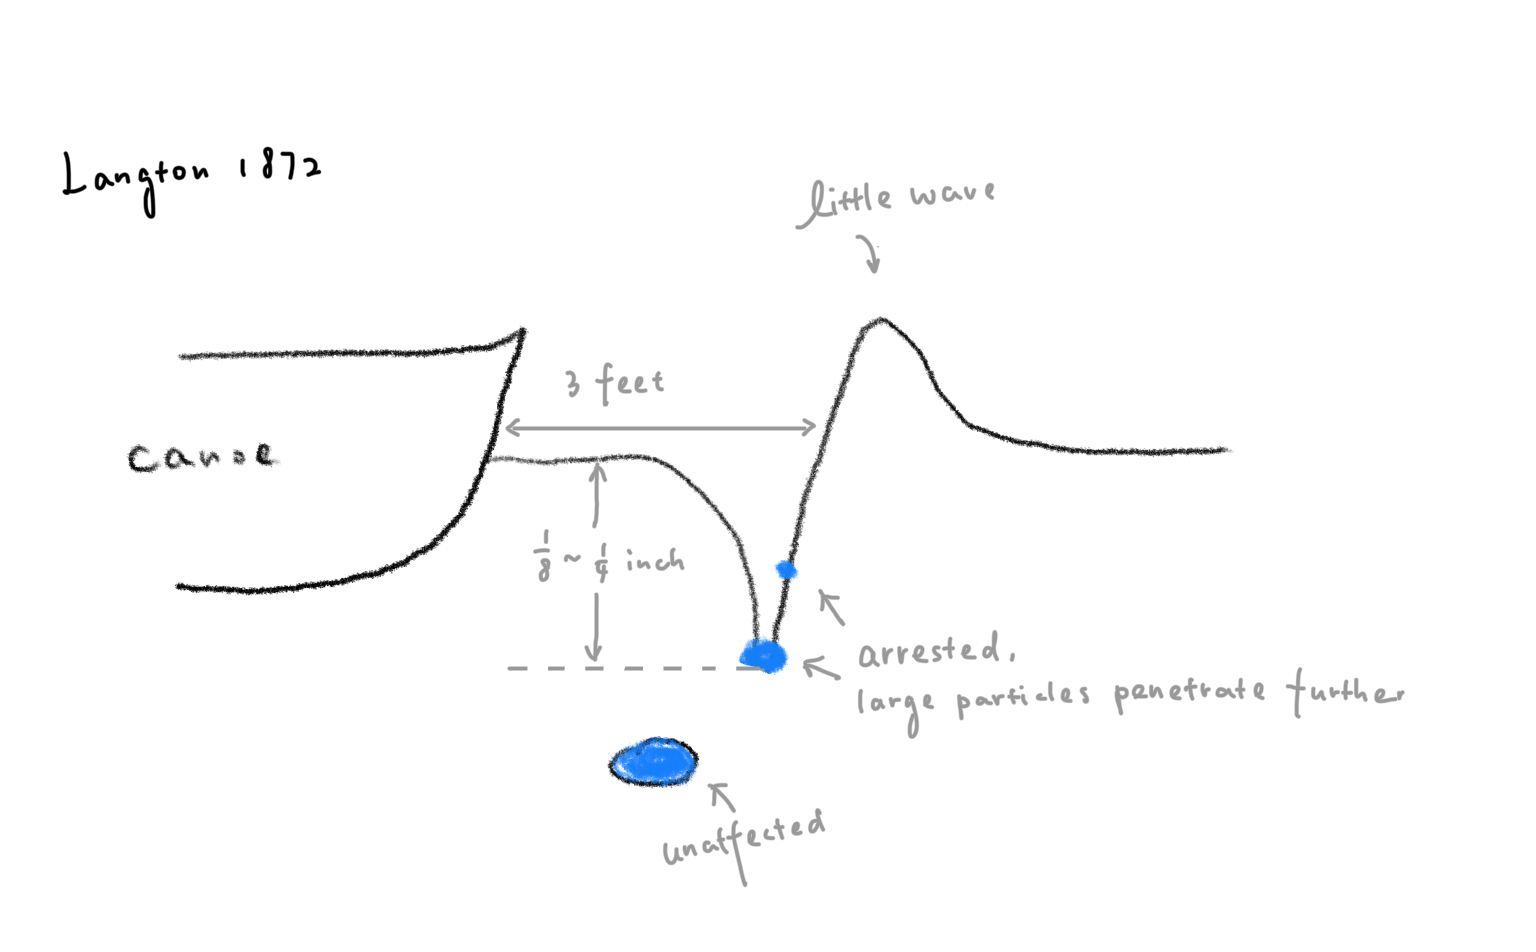
\includegraphics[width=\textwidth]{Figures/Langton 1872.png}
    \caption{A sketch based on Langton's description of the wave in front of his canoe.}
    \label{fig:Longton-1872}
\end{figure}


Here is a list of publications along with the key findings related to the Reynolds ridge:
\begin{itemize}
    \item Satterly (1919): \emph{Combustibility of mixtures of hydrogen and helium} \cite{Satterly1919};
    \item Burdon (1926): not found;
    \item Edser (1926): not found;
    \item Satterly \& Turnbull (1929): \emph{The ridge at the junction of clean and contaminated liquid surfaces} 
    \item Woog (1931): not found
    \item Schmidt (1936): \emph{Cause of Oil Patches on Water Surfaces} \cite{Schmidt1936}. ``The phenomenon is strikingly revealed as a moving reflection or refraction image when bright sunshine falls on to the bottom of the channel ... The same phenomenon is observed along the leeward shore of a lake ... where the wind-driven surface-water dives below a thin layer of slowly moving water.'' A picture of the moving reflection image at the bottom of a brook is shown in Fig.~\ref{fig:rr-examples}(a).
    \item Stansfield (1936): \emph{Line on the Surface of Water} \cite{Stansfield1936}. The author followed up \cite{Schmidt1936} by reporting the observations of the ``line'' in a drinking-trough, as well as in front of a moving raft (see Fig.~\ref{fig:rr-examples}(b) for a sketch made by the author). 
    \item Hall (1936): \emph{Lines on the Surface of Moving Water} \cite{Hall1936}. The author observed the ``line'' near a bridge that touched the water in a river. He also reported secondary waves, which were ``a series of parallel waves of diminishing amplitude and stationary with respect to the line''. See Fig.~\ref{fig:rr-examples}(c) for a photo.
    \item Burdon (1949): not found;
    \item Bell (1954): not found;
    \item Merson \& Quinn (1965): I do not find the original paper, but the references of \cite{Mockros1968} give an idea what this paper is about. ``Detailed study of the growth properties of such films was reported by Merson and Quinn ... Experiments with barriers of brass, plexiglass, and Teflon had shown that, despite differing menisci, film growth was unaffected by the various methods of touching the surface with the barrier.''
    \item Sellin (1968): \emph{Existence of a Surface Tension Discontinuity at a Liquid Free Surface} \cite{Sellin1968}. The author reports the first quantitative measurement of the "surface line" using a reflected light Schlieren system. 
    \item Mockros \& Krone (1968): \emph{Hydrodynamic Effects on an Interfacial Film} \cite{Mockros1968}. The authors reported observation of circulation in the surface film, as well as measurements of surface tension gradient and shear force. 
    \item McCutchen (1970): \emph{Surface Films Compacted by Moving Water: Demarcation Lines Reveal Film Edges} \cite{McCutchen1970}. He used the reflections of a fishline, as well as a wire screen, to visualize the water surface elevation. 
\end{itemize}

\begin{figure}
    \centering
    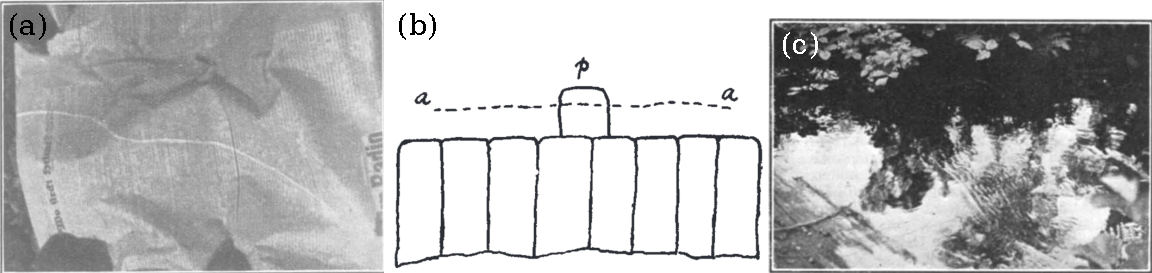
\includegraphics[width=\textwidth]{Figures/Reynolds-ridge-examples.pdf}
    \caption{(a) The "thread" image on the bottom of a stream (b) Sketch of the front end of the raft, a, a is the line on the surface. (c) The line near a bridge in a river, and the secondary waves }
    \label{fig:rr-examples}
\end{figure}

\section{Methods}

Several methods have been used to observe the distorted water surface near a Reynolds ridge, including the reflected light Schlieren system by Sellin \cite{Sellin1968}, reflections of fishlines and wire screens (objects with known shape) by McCutchen \cite{McCutchen1970}, and the direct observation with a straight-line light source by Scott \cite{Scott1982}. In this section, I review the principles of these methods.

\subsection{Reflected light Schlieren system}

Optical systems which make use of the refraction undergone by light transmitted through gases of varying density are known collectively as \emph{Schlieren systems}. Sellin used this technique to detect distortions at water surfaces. In this technique, a beam of light is brought to a precise focus by a primary lens. A stop is placed at this focus, so that normally no light is allowed to pass this focus to form an image on the photographic plate behind the focus. The light beam is also allowed to pass through the water surface. Normally, when the surface is quiescent, it serves as a mirror and brings all the light to the focus. When the surface is distorted, however, the deflected light gets around the stop and forms an image on the photographic plate. Fig.~\ref{fig:schlieren-system} shows a diagram of the Schlieren system.

\begin{figure}
    \centering
    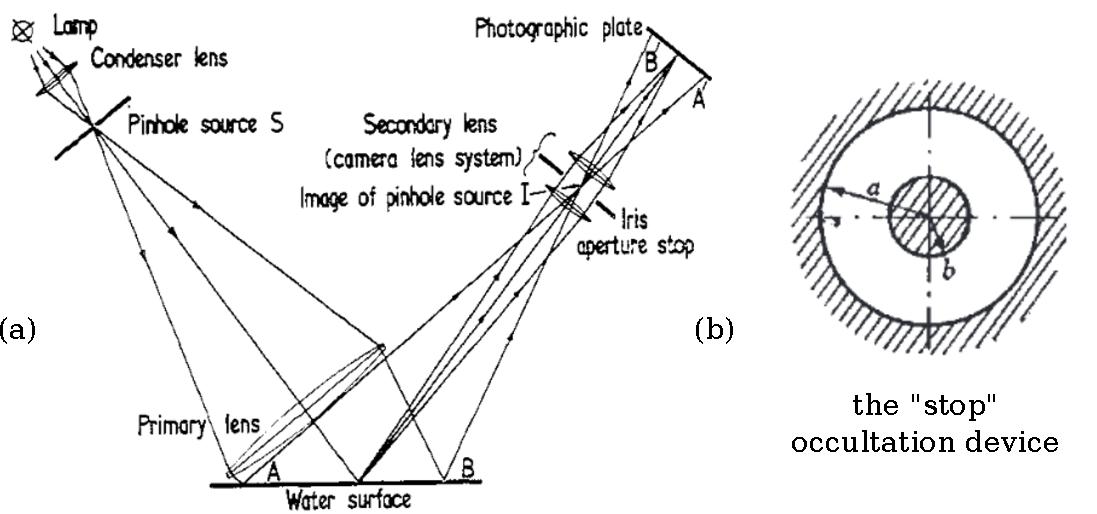
\includegraphics[width=\textwidth]{Figures/schlieren-system.pdf}
    \caption{Illustration of a Schlieren system. Reproduced from \cite{Sellin1963} and \cite{Sellin1968}.}
    \label{fig:schlieren-system}
\end{figure}

The results obtained by Sellin using the Schlieren system were criticized by Scott: ``the finite radius of the central opaque area means that a deflection has to be greater than the smallest central disk radius for it to be detected at all''. Consequently, surface features such as the gently sloping regions were missed. 

\subsection{Reflected straight lines}

McCutchen used the reflections of fishlines and wire screens as indicators of surface distortion. Compared to the Schlieren images, the reflections used in this method give a relatively direct representation of the surface profile. The result is shown in Fig.~\ref{fig:reflected-straight-lines}. 

\begin{figure}
    \centering
    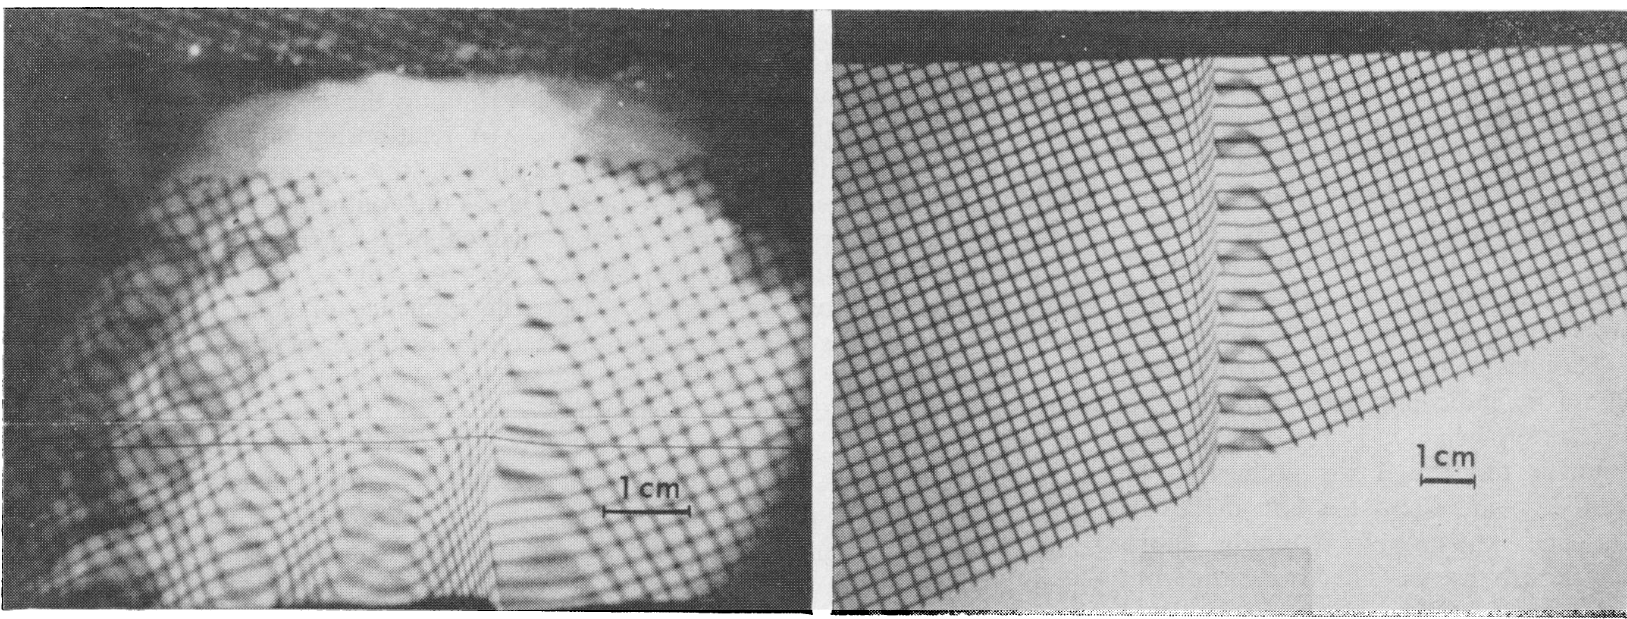
\includegraphics[width=\textwidth]{Figures/reflection-straightline.png}
    \caption{Reflections of a straight fishline and a wire screen under Reynolds ridge. Reproduced from \cite{McCutchen1970}.}
    \label{fig:reflected-straight-lines}
\end{figure}

Scott pointed out, however, that such images do not uniquely define the surface slope. Gilbert found that for a fixed orientation of the apparatus, more than one surface can give rise to a given observed image \cite{Gilbert1980}. It is possible to overcome the non-uniqueness problem by taking two photos at different angles.

\subsection{Direct observation with a straight-line light source}

Scott made direct observation of water surface profile with a straight-line light source. Taking photos from both upstream and downstream of the Reynolds ridge, he observed different profiles, which turned out to be approximate inversions of each other (see Fig.~\ref{fig:straightline-light-source-images}). I am still struggling to understand the explanation by Scott for why the image from upstream appear to be the inversion of the image from downstream.

\begin{quotation}
(from Scott 1982 \cite{Scott1982})

The shape of the observed image distortion in this arrangement is seen to be approximately inverted by the change of observation point from upstream to downstream. Of the three surface-shape parameters which might be considered to have a significant effect on the observed image - the vertical displacement, the surface slope and the surface curvature - only the slope is expected to give an image distortion that is an odd function of the observation direction. It may thus be intuitively reasonable to deduce that the slope variation may have at least a major effect on the image distortion in the present case. 

In a case such as this, the following line of reasoning is found to be valid. When visual observation is from a given direction, the image is observed to be displaced upwards if the corresponding part of the surface is inclined upwards towards the observer, and displaced downwards if the surface slopes downwards away from the observer. Obviously, when the observer changes his position from one side of the surface distortion tothe other side, any part of the surface originally inclined upwards now appears inclined downwards, and the image is indeed seen to change accordingly.
\end{quotation}

\begin{figure}
    \centering
    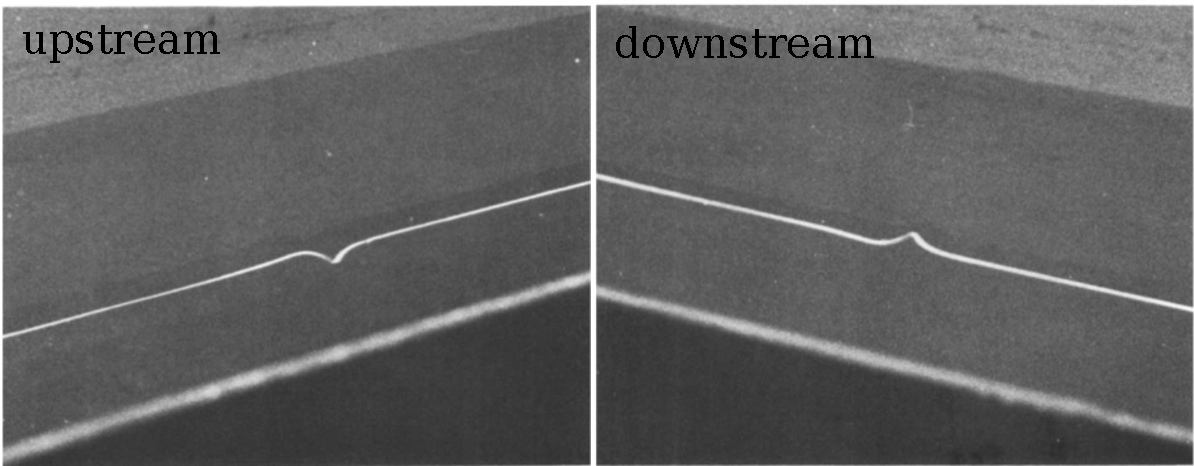
\includegraphics[width=\textwidth]{Figures/straightline-light-source-images.pdf}
    \caption{Images of Reynolds ridge illuminated by a straight-line light source, (a) looking from upstream and (b) looking from downstream.}
    \label{fig:straightline-light-source-images}
\end{figure}

\section{Research plan}

\subsection{Is it Reynolds ridge?}

The objective of the present work is to understand the fringes around soaked porous objects, such as pickled beet root and dumplings in soy sauce (Fig.~\ref{fig:beet-and-dumplings}). Are they merely an instance of Reynolds ridge, which results from the competition between an expanding surface film and a compressing viscous drag underneath?

\begin{figure}
    \centering
    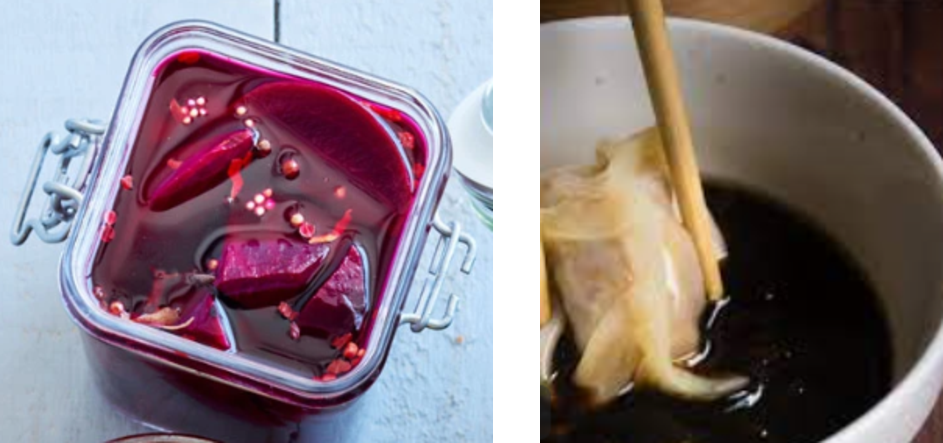
\includegraphics[width=0.8\textwidth]{Figures/beet-and-dumplings.pdf}
    \caption{Pickled beet root and dumplings in soy sauce.}
    \label{fig:beet-and-dumplings}
\end{figure}

As I read more about Reynolds ridge, I get more skeptical that the fringes we are concerned may not be an example of Reynolds ridge, but something else. An important clue is the absence of the flow underneath. Even if there does exist a tiny flow due to the object being porous, the flow rate would be too small to induce a Reynold ridge very close to the object. Recall that in the Reynolds ridge case, higher flow rate results in the ridge closer to the barrier, while vanishing flow rate results in free spreading of contaminants, making the ridge disappear.

So in my opinion, Scott mistakenly cited Satterly 1956 \cite{Satterly1956} as an observation of a Reynolds ridge. 

\subsection{Create and characterize the fringe}

We hypothesize that the fringes around beet roots and dumplings are due to these object being porous. We could have done the experiment with beet roots or dumplings for sure, but having \emph{a simpler and more controlled material} would benefit future studies. 

Therefore, I will start my experiment with porous material fabrication. The idea is to have a systematic control of the pore size and density of the same material, so we can investigate the effects on liquid film distortion.

Then, I need to look for a liquid which is ideal for the confocal surface profiling. To do this, I have to do the training and consult the expert for advice.

Nonetheless, our investigation can start with two measurements:
%
\begin{itemize}
    \item Fluid motion under the surface of the fringe
    \item Surface profile
\end{itemize}
%
Some existing theories are worth reading and working out:
%
\begin{itemize}
    \item \emph{The Deduction of Surface Profiles from the Reflection of Horizontal-line Light Sources: Calculation of the surface profile} \cite{Gilbert1980}: to deduct surface profiles from images using optic principles.
    \item \emph{he leading edge of a surface film on contaminated flowing water} \cite{Harper1974}: to derive the surface profile of Reynolds ridge using hydrodynamic principles.
\end{itemize}

I also notice in Satterly 1956 \cite{Satterly1956} another interesting phenomenon: when leaving a salt solution to evaporate in a beaker, the salt solid climbs inches up the sides of the beaker. This reminds me of \emph{tears of wine}, which is a result of surface tension driven flow (or Maragoni effect, see Fig.~\ref{fig:tears-of-wine}). When the bulk liquid is thin, it is possible that Maragoni effect can induce a distortion near the meniscus.

\begin{figure}
    \centering
    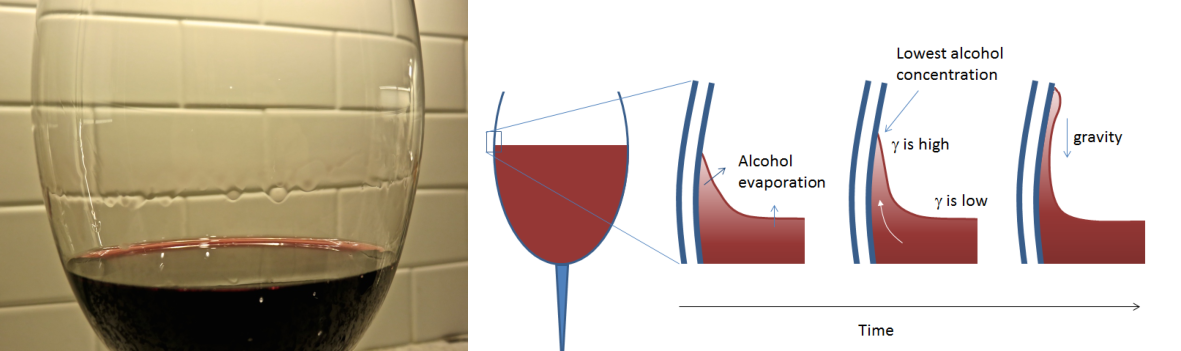
\includegraphics[width=\textwidth]{Figures/tears-of-wine.pdf}
    \caption{Tears of wine caused by Maragoni effect.}
    \label{fig:tears-of-wine}
\end{figure}

\section{Surface profile}

After arriving at Cornell, I was able to actually measure the surface profiles of the thin film around porous objects, e.g. beet root.
This is my first surface profile measurement (04/04/2024).
I used the \textit{Keyence displacement sensor} to measure the surface profile. A schematic and a photograph are shown in Fig.~\ref{fig:surface-profiling}. 
This tool turns out to be very precise: it is capable of measuring changes of surface height down to 0.25 $\mu$m, while the temporal resolution is above 1000 Hz. 
These resolutions are more than enough for our application, which is measuring a quasi-stationary surface profile. 
In this section, I present some preliminary measurements of the surface profiles around beet root, styrofoam and rubber. 
These measurements suggest some possible improvement that could be made to the current setup: a motorized linear stage and a perfectly flat bench. 

\begin{figure}
    \centering
    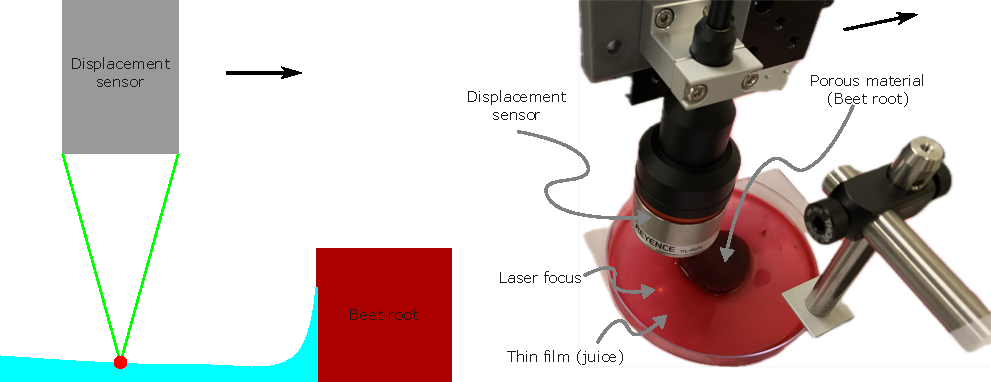
\includegraphics[width=\textwidth]{Figures/surface_profiling.pdf}
    \caption{A schematic of the Keyence displacement sensor (left) and a photograph of the tool in a measurement.}
    \label{fig:surface-profiling}
\end{figure}

\subsection{Surface profile measurement}

In the first measurement, I tested three materials (beet root, styrofoam and rubber) and two film thicknesses (thin and thick). 
The results, focusing on whether the white bands show up (or abnormal distortion of the surface), are summarized in Table.~\ref{tab:surface-profile-result}.

\begin{table}
    \centering
    \begin{tabular}{c|ccc}
        \hline
                   & Beet   & Styrofoam & Rubber \\
        \hline 
        Thin film  & \cmark & \cmark    & \xmark \\
        Thick film & \xmark & \xmark    & \xmark \\
        \hline
    \end{tabular}
    \caption{``White band'' result summary.}
    \label{tab:surface-profile-result}
\end{table}

Thin film surface profiles are shown in Fig.~\ref{fig:thin-film-surface-profile}.
In the plots, the surface profile starts from the solid object at $x=0$.
Vertically, $y=0$ is defined as the lowest point of the surface profile.
Both beet root and styrofoam induce a valley between solid and the liquid film far away, while in the rubber test we barely observe such valley.
This observation supports the hypothesis that porous materials are responsible for the surface distortion of the thin film. 

The valley appears at different distances from the solid objects. 
For beet root, the valley typically appears 6 mm away.
For styrofoam, however, the valley typically appears less than 1 mm away, which is much closer. 
Pore size may be responsible for this difference.

\begin{figure}
    \centering
    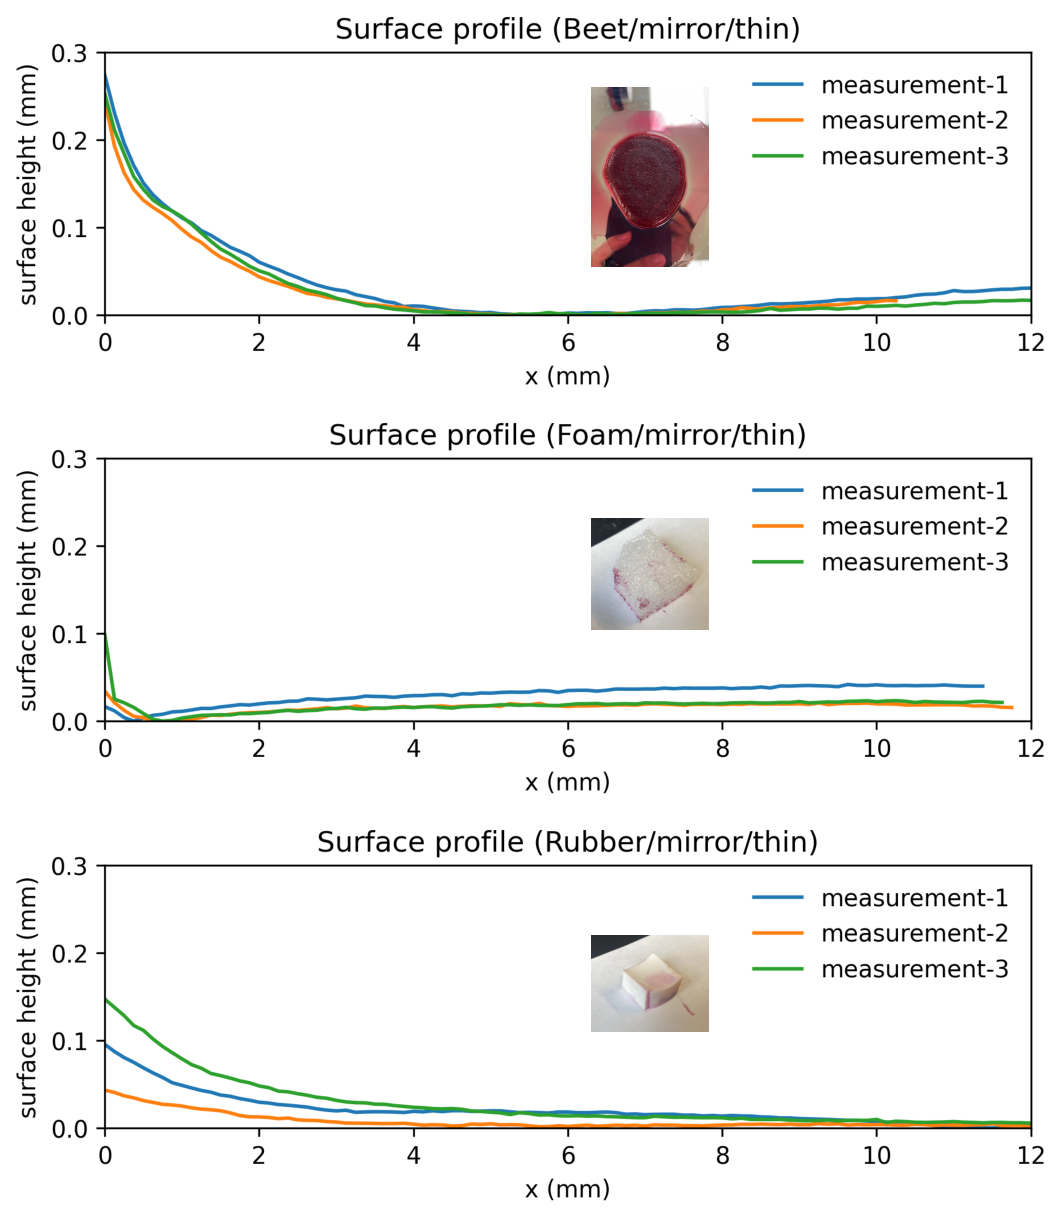
\includegraphics[width=\textwidth]{Figures/surface_profile_measurement_mirror_04042024.pdf}
    \caption{Thin film surface profiles around beet root, styrofoam and rubber.}
    \label{fig:thin-film-surface-profile}
\end{figure}

Thick film surface profiles are shown in Fig.~\ref{fig:thick-film-surface-profile}.
All the profiles, no matter what solid material is used, show monotonic decreasing height. 
This suggest the ``white band'', i.e. the abnormal surface distortion, occurs only when the film is sufficiently thin.

\begin{figure}
    \centering
    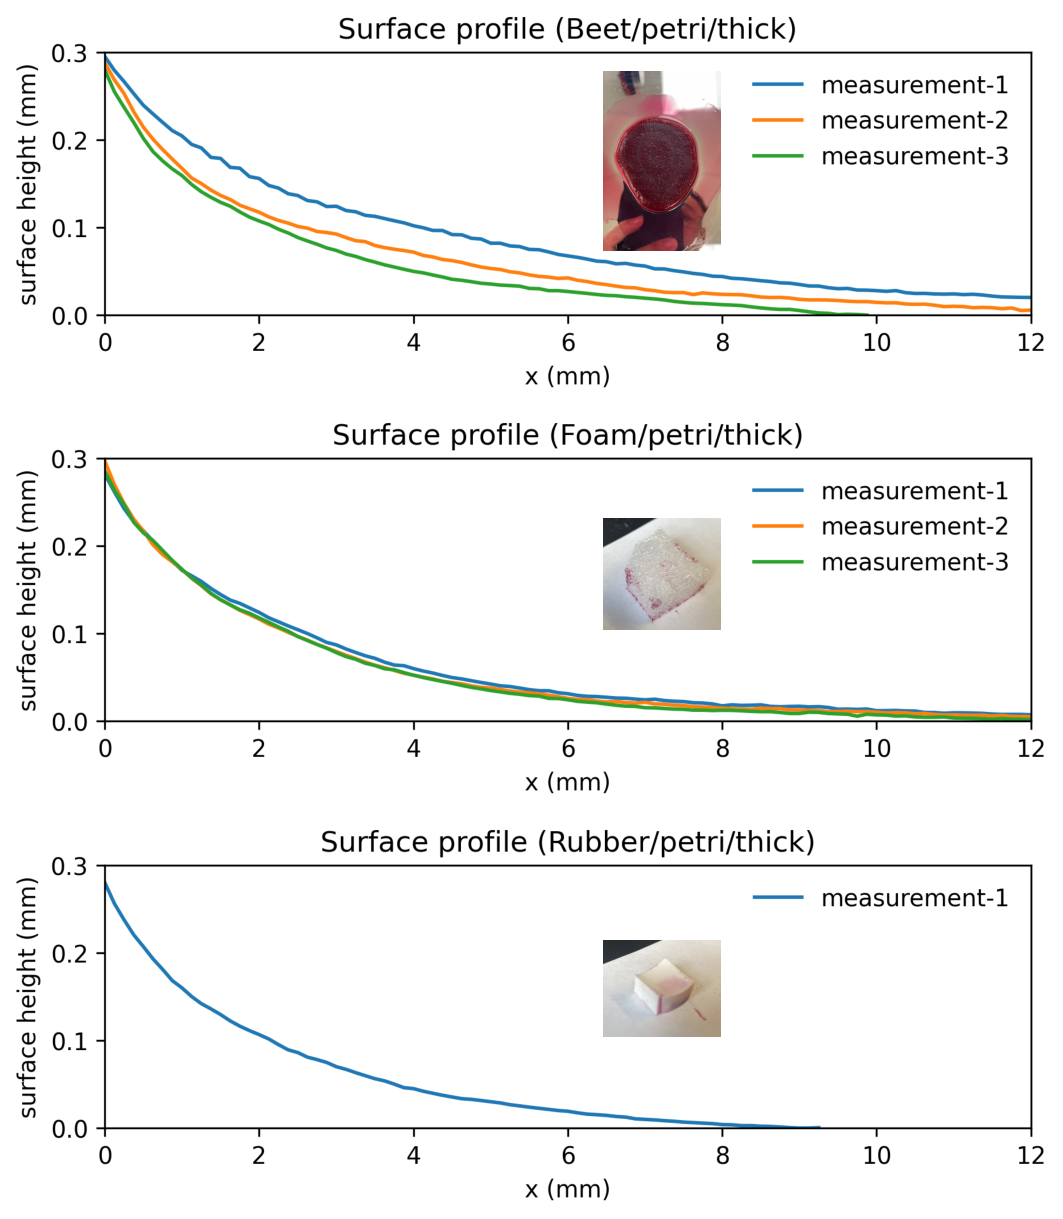
\includegraphics[width=\textwidth]{Figures/surface_profile_measurement_petridish_04042024.pdf}
    \caption{Thick film surface profiles around beet root, styrofoam and rubber.}
    \label{fig:thick-film-surface-profile}
\end{figure}

\subsection{Beet root drying time-lapse}

To see whether evaporation is the cause of the fringe, I did a drying experiment of beet root soaked in juice in a petri-dish. The experiment was recorded with GoPro camera in time-lapse mode. Some snapshots (8/177) are shown in Fig.~\ref{fig:beet-juice-drying-timelapse}. The drying of the juice took about 150 minutes, after which the beet root started to lose water and shrank. A white fringe can be observed in the images, whose upper boundary follows the shape of petri-dish boundary, and whose lower boundary follows the shape of the beet root. However, I believe that this is not the fringe we usually observe, but is due to the meniscus bridge between the beet root and the petri-dish side wall. At the end of the video, we observe a lot of red stain deposited at the bottom of the petri-dish. 

\begin{figure}
    \centering
    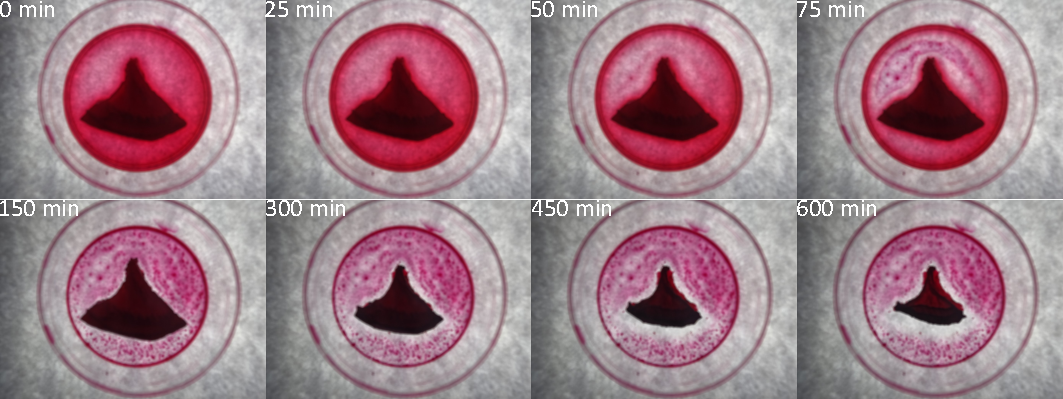
\includegraphics[width=\textwidth]{Figures/beet-juice-drying-timelapse.pdf}
    \caption{Beet juice drying time lapse.}
    \label{fig:beet-juice-drying-timelapse}
\end{figure}

\subsection{Improving the measurement}

The current measurement poses a few problems, which could be improved:
\begin{itemize}
    \item The horizontal scan is achieved by manually twisting the screw of a micromanipulator. Manual control means that the speed of scan is not 100\% uniform, which further suggests that the horizontal locations in the surface profile plots are not accurate. To solve this problem, we can motorize the micromanipulation to guarantee a constant speed of scan. \textcolor{magenta}{We have a motorized linear stage now, which can move at a constant speed $v\approx 1.6$ mm/s.}
    \item The substrate is not perfectly flat. As a result, the film on one side may be thinner than the film on the other side. See Fig.~\ref{fig:surface-profiling} right panel for an example, where the upper part of the petridish is higher, resulting in a thinner film. To solve this problem, we can add a substrate below, of which the tiltedness can be adjusted. \textcolor{magenta}{Sunny suggests to float the substrate on water, but I have not come up with a very feasible plan yet. On the other hand, substrate being not flat does not affect the measurement much, so for now I will live with the tiltedness, which is about 0.2$^\circ$.}
    \item The juice of beet root, when evaporated, leaves solid precipatates on the substrate. Figure~\ref{fig:beet-juice-drying-timelapse} is a time-lapse of beet juice drying, in which the precipatates can be clearly seen. They can then mix with the liquid film, and generate confusing surface profile (typically with an unexpected peak). Due to this reason, pure water may be a better alternative compared to the juice. \textcolor{magenta}{I tried pure water but was not able to see the ``dimple''. Water does not wet the mirror surface very well, compared to beet juice. I have not tried to induce the dimple with fluid motion, but I think I should try next time.}
\end{itemize}



\section{Surface profile 2}

In this section, we record the second measurement with the Keyence distance sensor (04/10/2024). This time, I improved the setup with a motorized stage, allowing more efficient and accurate surface profile measurement. I also make bevel on all the three materials tested, to avoid expected light blocking before the whole surface is measured. In addition to beet juice, I tried pure water to see if this phenomenon is specific to certain fluid. I also did a fix point long time measurement at the dimple, to see if it is a transient phenomenon. Detailed results follow.

\subsection{Motorized stage}

The motorized stage in our lab turned out to be the same model as the stage in the Roh lab for the distance sensor. Therefore, the upgrading of the setup to a motorized distance sensor is not difficult. Fig.~\ref{fig:motorized_stage_for_distance_sensor} shows the distance sensor setup with the mounted on the motorized stage. 

\begin{figure}
    \centering
    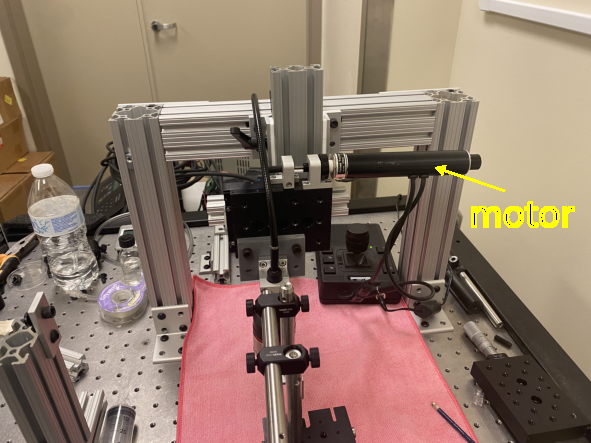
\includegraphics[width=0.6\textwidth]{Figures/motorized_stage_for_distance_sensor.pdf}
    \caption{Keyence distance sensor mounted on a motorized stage.}
    \label{fig:motorized_stage_for_distance_sensor}
\end{figure}

\subsection{Water test}

In the last experiment, we saw the potential influence of the beet juice deposits to the surface profile measurement. This time, therefore, we use water as the liquid phase and see if it produces similar fringe pattern (thin film). The result is shown in Fig.~\ref{fig:surface_profile_water_test_04102024}. No ``dimple'' was observed. And the liquid film was much shorter compared to the film of beet juice. The front mirror was quite hydrophobic, and it seemed impossible for water to form a thin film on it. On the contrary, the beet juice can easily wet the mirror and form thin film. The fact that the juice wets the front mirror so well suggests that there might be surfactant in it. And if so, that constitutes one condition for \emph{Reynolds ridge} to form. 

Note that I also tried to tilt the mirror to make water flow around the solid. That did not result in successful ``dimple'' formation because of the hydrophobicity of the mirror.
\begin{figure}
    \centering
    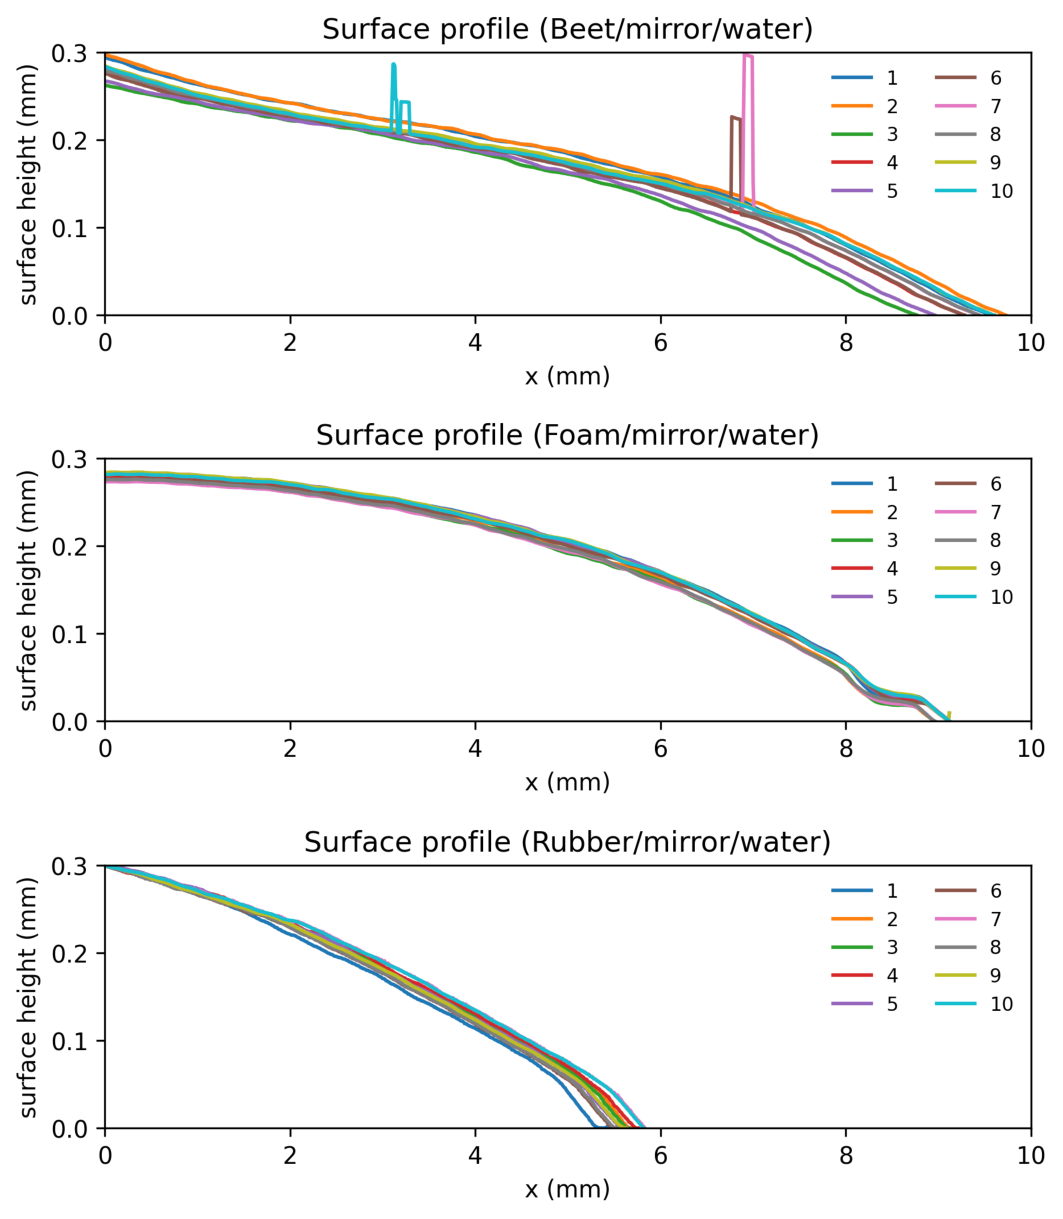
\includegraphics[width=\textwidth]{Figures/surface_profile_water_test_04102024.pdf}
    \caption{Surface profiles of water on front mirror around beet root, styrofoam and rubber.}
    \label{fig:surface_profile_water_test_04102024}
\end{figure}

\subsection{Beet juice test}

With motorized scanner, we measure the surface profile of beet juice around beet root again. Motorized setup allows more efficient and consistent measurement of the surface profile. The results of 10 measurements are shown in Fig.~\ref{fig:surface_profile_measurement_mirror_juice_04102024}. before measurement 1 and 6, I tilted the mirror to generate some flow of the juice, which made the ``dimple'' much more obvious. The surface measurements for 1 and 6 indeed show that there is a thinner region between the bulk of the juice film and the beet root. The subsequent measurements show no such ``dimple'' feature, suggesting that this is a transient phenomenon caused by the fluid flow. 

\begin{figure}
    \centering
    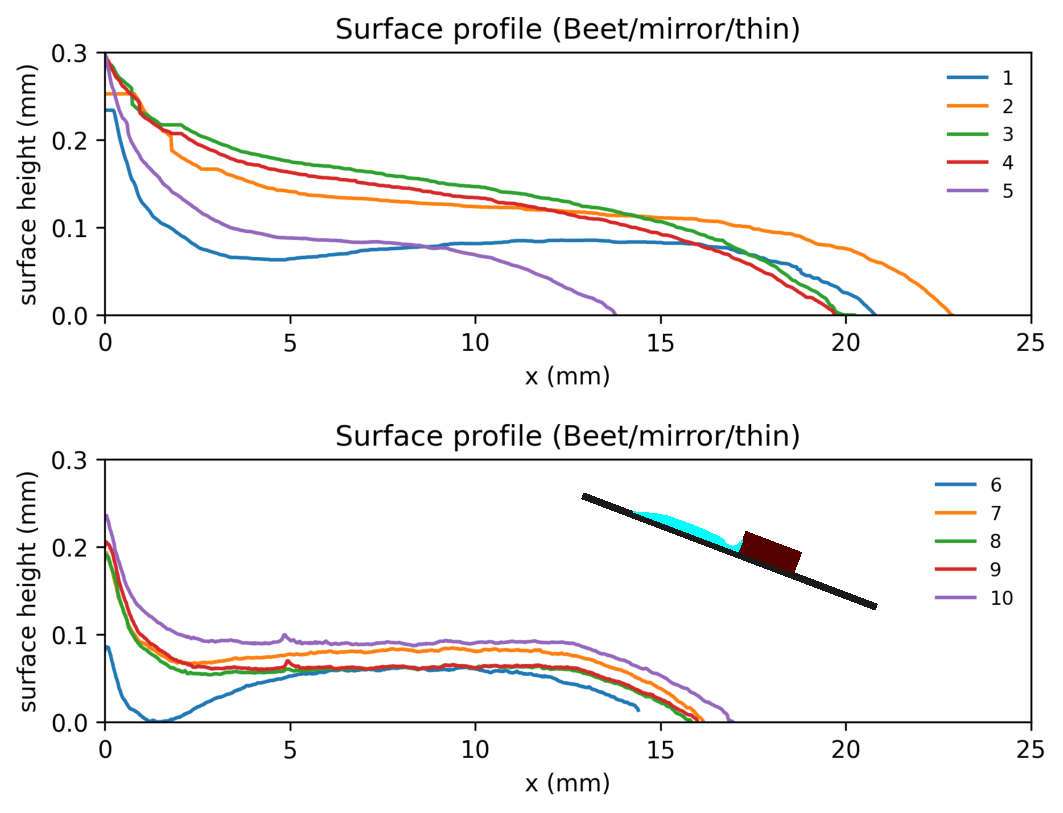
\includegraphics[width=\textwidth]{Figures/surface_profile_measurement_mirror_juice_04102024.pdf}
    \caption{Surface profiles of beet juice around beet root on front mirror. The 10 measurements are done on the same sample, but the profiles are not consistent. Note that before measurement 1 and 6, I tilted the mirror to generate some flow of the juice, which made the ``dimple'' much more obvious. After about a minute, the ``dimple'' disappeared.}
    \label{fig:surface_profile_measurement_mirror_juice_04102024}
\end{figure}

\subsection{Fixed point long time measurement}

To further verify that the ``dimple'' is transient, we fixed the distance sensor at the ``dimple'' and measure how the height of surface evolved over time. The result is shown in Fig.~\ref{fig:fixed_point_long_time}. Right before the data recording, I tilted the mirror to generate some flow, so that the ``dimple'' appeared. The data show that the surface rose in the first 100 seconds by about 0.16 mm. Then the surface fell at a much lower rate (about 80 times slower). The rise is likely caused by compensating fluid flow due to either gravity or surface tension. And the fall is likely due to evaporation.

\begin{figure}
    \centering
    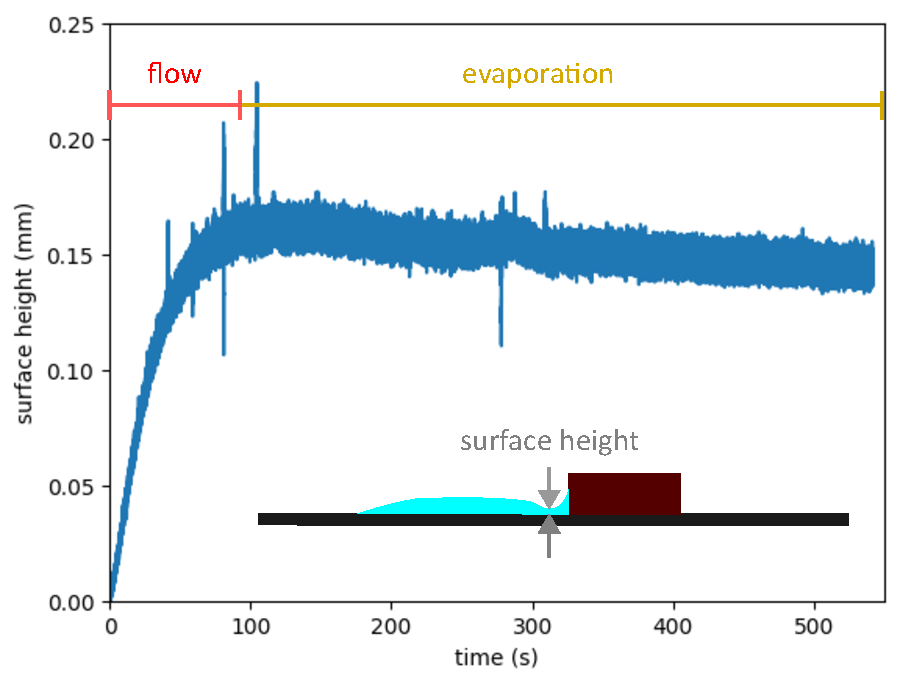
\includegraphics[width=0.6\textwidth]{Figures/fixed_point_long_time.pdf}
    \caption{Temporal evolution of surface height at the ``dimple''.}
    \label{fig:fixed_point_long_time}
\end{figure}

\subsection{Things to be improved}

This data set presents some things to be improved:

\begin{itemize}
    \item baseline: in the current data, the baseline is arbitrarily defined as the lowest point of the cropped surface profile. This limits us from appreciating the real temporal evolution of the surface, due to either relaxation or evaporation. This can be improved by zero the measurement carefully before experiment.
    \item contact line: use the ``rub'' technique to generate flow, rather than tilting the substrate. This can help avoid disturbing the pinned contact line. Always start measurement from contact line.
    \item use fluid dye when testing colorless liquid.
\end{itemize}

\section{Surface profile 3}

This section summarizes the surface profile measurement on 04/18/2024. To test the surface tension effect, I use liquids with different surface tension and measure the surface profiles of each forming around solid objects (beet/sponge/rubber). To acquire more replicates, I also employed a new method of scanning the same surface back and forth. In this way, I minimize and standardize the time interval between each scan, and hopefully make replicates more reliable. We summarize the result here and discuss the message we learn. 

While we have some hundreds of scans in total, here I only show the average of each combination for space consideration. The results are shown in Fig.~\ref{fig:different-liquid-all-in-one_04182024}. 

\begin{figure}
    \centering
    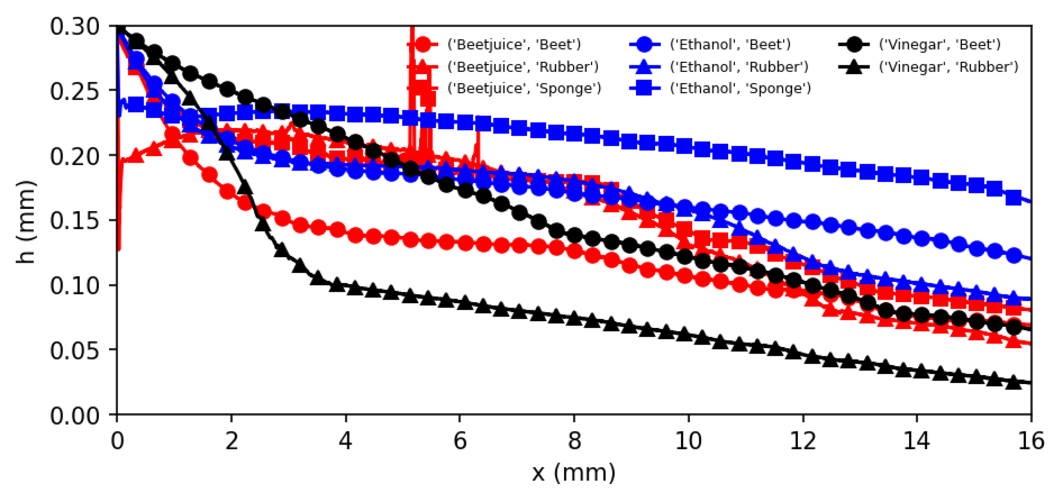
\includegraphics[width=0.8\textwidth]{Figures/different-liquid-all-in-one_04182024.pdf}
    \caption{All combinations surface profiles.}
    \label{fig:different-liquid-all-in-one_04182024}
\end{figure}

The most outstanding feature of this data set is that all the profile scans show a consistent angle with respect to the horizontal axis. This angle is small. A rough estimate indicates that it is no larger than 0.3$^\circ$. However, it can substantially change how we interpret the data, in particular, whether we observe the dimple or not. Figure~\ref{fig:impact_of_nonflat_scan} shows an example of how a nonflat scan can impact our interpretation. The black line is the original surface to be measured, and no dimple is present in that surface. However, if our scan is tilted (either the bottom substrate or the displacement sensor holder, as sketched in the inset), we end up with the red line, which is simply a rotated version of the black line, but shows a dimple. In next experiment, I am going to carefully adjust the scanner holder to minimize this angle.

\begin{figure}
    \centering
    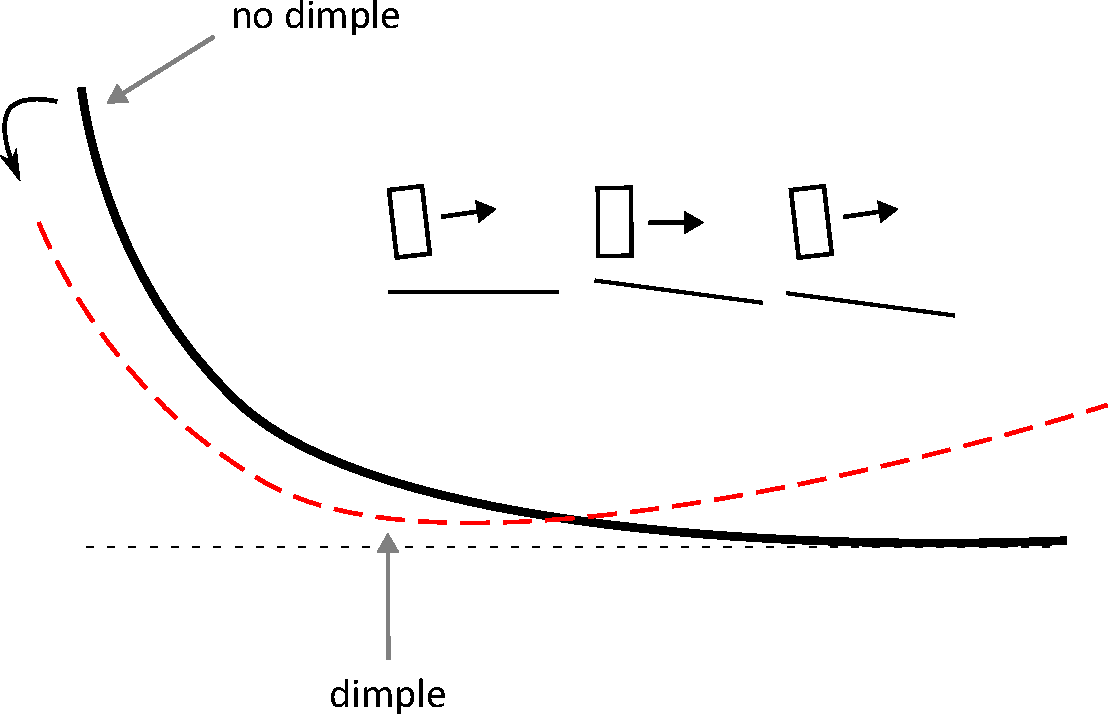
\includegraphics[width=0.6\textwidth]{Figures/impact_of_nonflat_scan.pdf}
    \caption{Impact of nonflat scan.}
    \label{fig:impact_of_nonflat_scan}
\end{figure}

\section{Surface profile 4}
This section summarizes the surface profile measurement on 04/22/2024. Only beet and beet juice (fresh) are used. The highlight of this data is that the angle has been fixed by careful adjustment. The result of the adjustment can be seen in Fig.~\ref{fig:holder_adjustment}. Both curves are surface height scans for the mirror substrate. The blue line is before the adjustment and the orange line is after the adjustment. The tilted angle is reduced from $0.25^\circ$ to $0.02^\circ$. The increment of height over typical scan range (16 mm) reduces from 0.07 mm to 0.005 mm. 

\begin{figure}
    \centering
    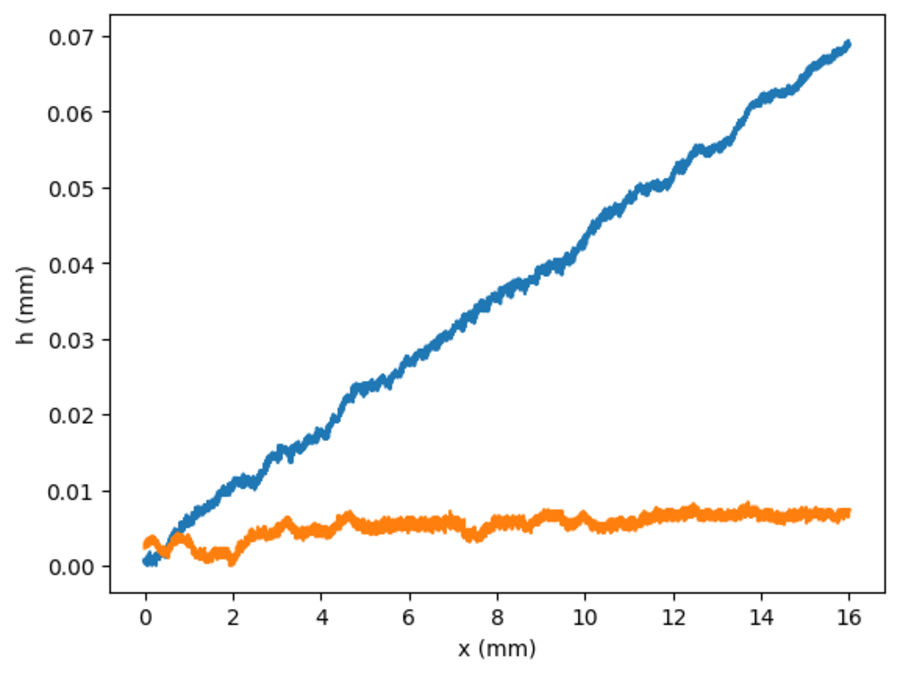
\includegraphics[width=0.6\textwidth]{Figures/holder_adjustment.pdf}
    \caption{Adjust holder to make substrate scan horizontal.}
    \label{fig:holder_adjustment}
\end{figure}

\subsection{Surface profile measurement}
With this improvement, we present the new measurement of the surface profiles of beet juice next to beet. The data is shown in Fig.~\ref{fig:beet_in_juice_dimple_04222024}. A dimple can be observed around $x=4$ mm. Note that this profile is an average over 40 scans, and some of the scans do not show dimple due to surface relaxation. The fact that the dimple shows up in the average profile is a convincing evidence that the thin liquid film get distorted due to the presence of the beet. 

\begin{figure}
    \centering
    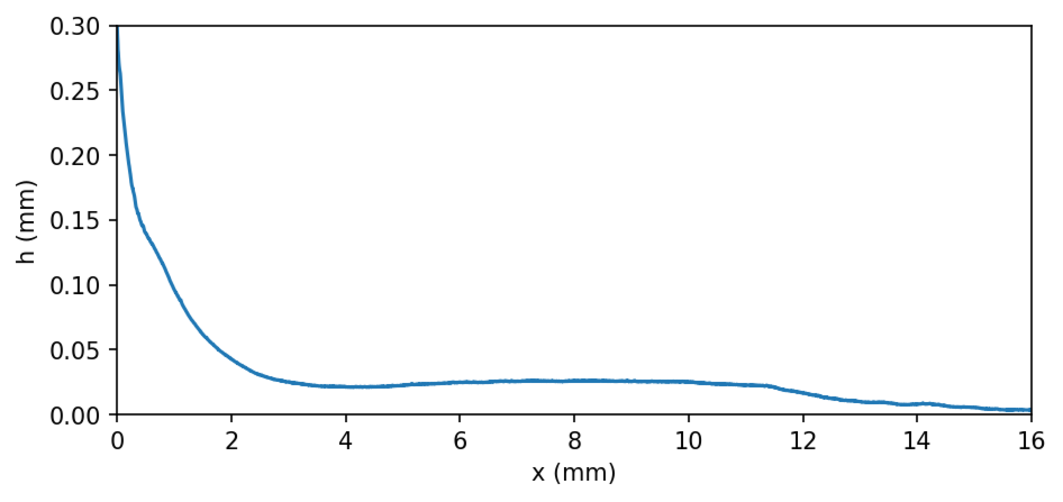
\includegraphics[width=0.8\textwidth]{Figures/beet_in_juice_dimple_04222024.pdf}
    \caption{Averaged surface height profile of beet juice around beet.}
    \label{fig:beet_in_juice_dimple_04222024}
\end{figure}

\subsection{Observation of flow}

A closer view of the thin layer around beet reveals a persistent flow going towards beet when beet is in contact with the juice. See Fig.~\ref{fig:flow_around_beet} for a snapshot and \href{https://drive.google.com/open?id=15En0p7fjopaUQokh8Cz-kZCVPX3ptZaZ&usp=drive_fs}{here for a preliminary video}. The small particles in the juice helps visualize the flow. The beet can surprisingly soak up a large amount of juice. 

\begin{figure}
    \centering
    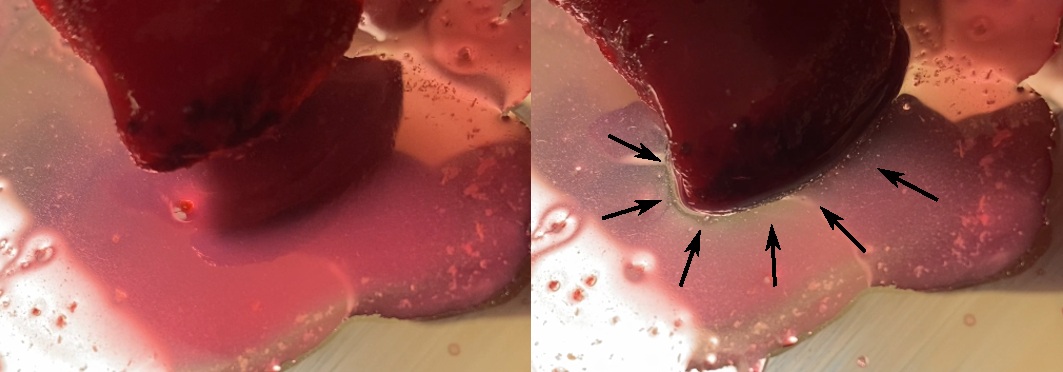
\includegraphics[width=0.8\textwidth]{Figures/flow_around_beet.pdf}
    \caption{Flow around beet.}
    \label{fig:flow_around_beet}
\end{figure}

I believe that the flow is the direct cause of the fringe pattern we have been observing around the beet. However, it is still not clear what is the mechanism behind the firnge. We can have hypotheses:

\begin{itemize}
    \item it is a Reynolds ridge, where incoming fluid flow compresses a surfactant film at fluid surface;
    \item the suction flow rupture the thin film around the beet;
    \item other possibilities. For example, depending on the thickness of the liquid film, different mechanisms can come into play. 
\end{itemize}

To better understand this fringe, we can do detailed measurement on the fluid flow and pressure. We can also use different theories based on different hypotheses to see which one agrees better with experiment.

\section{Flow measurement}

To measure the flow around the beet more accurately, I make the setup shown in Fig.~\ref{fig:flow_setup}.

\begin{figure}
    \centering
    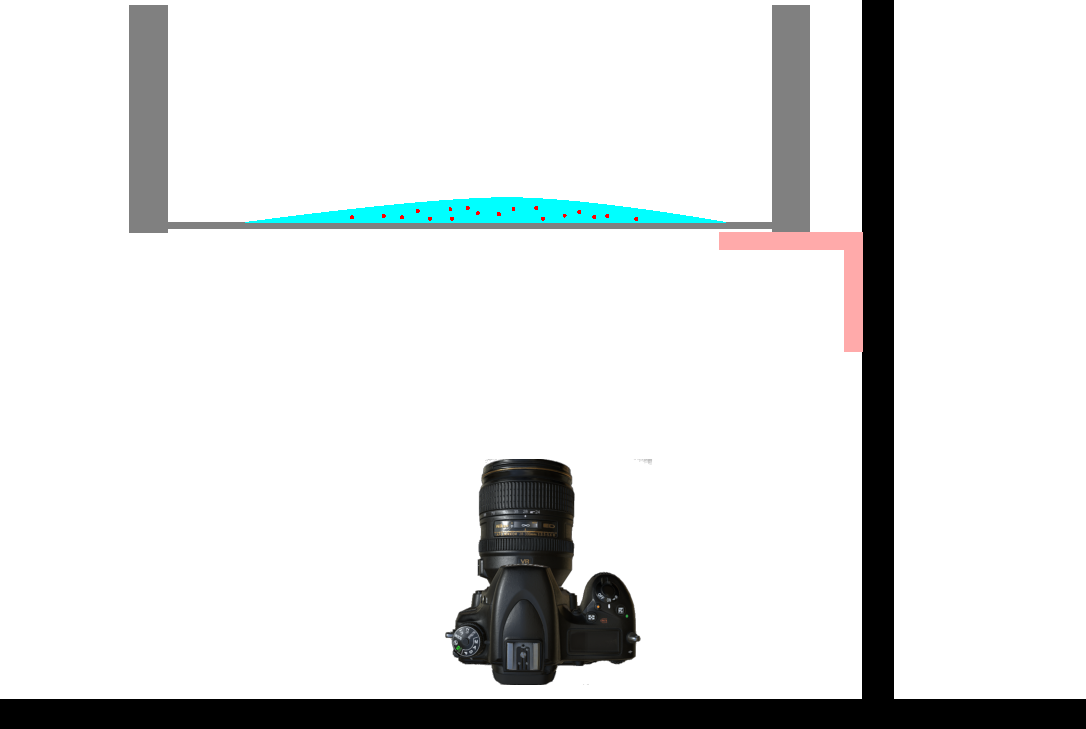
\includegraphics[width=0.8\textwidth]{Figures/flow_setup.pdf}
    \caption{Flow field measurement setup.}
    \label{fig:flow_setup}
\end{figure}

\newpage
\bibliographystyle{unsrt} 
\bibliography{refs}

\end{document}
